\section{Method}
\label{sec:method}

\noindent\textbf{Assumptions.}
Following the local-consistency assumption of
Voxgraph~\cite{reijgwart2020voxgraph}, we assume that TSDF fusion under the
drifted pre-correction trajectory remains locally valid: surface geometry and
connectivity are coherent in local neighborhoods although the map is globally
inconsistent. WarpVox corrects this global inconsistency after loop closure;
severely noisy or topologically corrupted source maps are outside its scope.

\subsection{Problem and Streaming State}

Let $T_i^- ,T_i^+\in SE(3)$ map sensor frame $S_i$ to the world frame before
and after trajectory correction. The map built with $\{T_i^-\}$ consists of a
TSDF $\Phi^-$, its weight field $w^-$, voxel size $s$, and truncation distance
$\tau$. Marching Cubes (MC)~\cite{10.1145/37402.37422} extracts the source
surface $\mathcal M^-=(V^-,F)$.

During fusion, WarpVox retains timestamped sensor-frame surface samples in a
bounded state indexed by the active TSDF cells $\mathcal A$:
\begin{equation}
\mathcal S=\{\mathcal S_c\}_{c\in\mathcal A},
\qquad |\mathcal S_c|\le n_c.
\label{eq:streaming_state}
\end{equation}
After surface extraction, each vertex queries a fixed neighboring-cell stencil
and applies the geometric validation below. We write this Stage-1 resolution as
\begin{equation}
\begin{aligned}
\mathcal O&=\mathcal R(\mathcal M^-,\{T_i^-\},\mathcal S),\\
\mathcal O_j&=\{(t_i,m_{ij},\alpha_{ij})\},
\qquad |\mathcal O_j|\le n_v,
\end{aligned}
\label{eq:resolved_records}
\end{equation}
where $m_{ij}$ is expressed in $S_i$ and $\alpha_{ij}\in[0,1]$ is the
effective reliability of the retained association. Records are matched by
acquisition time rather than trajectory row index. Thus the online state is
cell-indexed, while the correction backend receives bounded vertex-indexed
records without retaining the range stream:
\begin{equation}
(\Phi^-,w^-,\mathcal M^-,\{T_i^+\},\mathcal O)
\longmapsto (\Phi^+,w^+).
\label{eq:contract}
\end{equation}
The warped mesh is intermediate; $(\Phi^+,w^+)$ is the returned
Voxblox-compatible TSDF.

\begin{figure}[t]
  \centering
  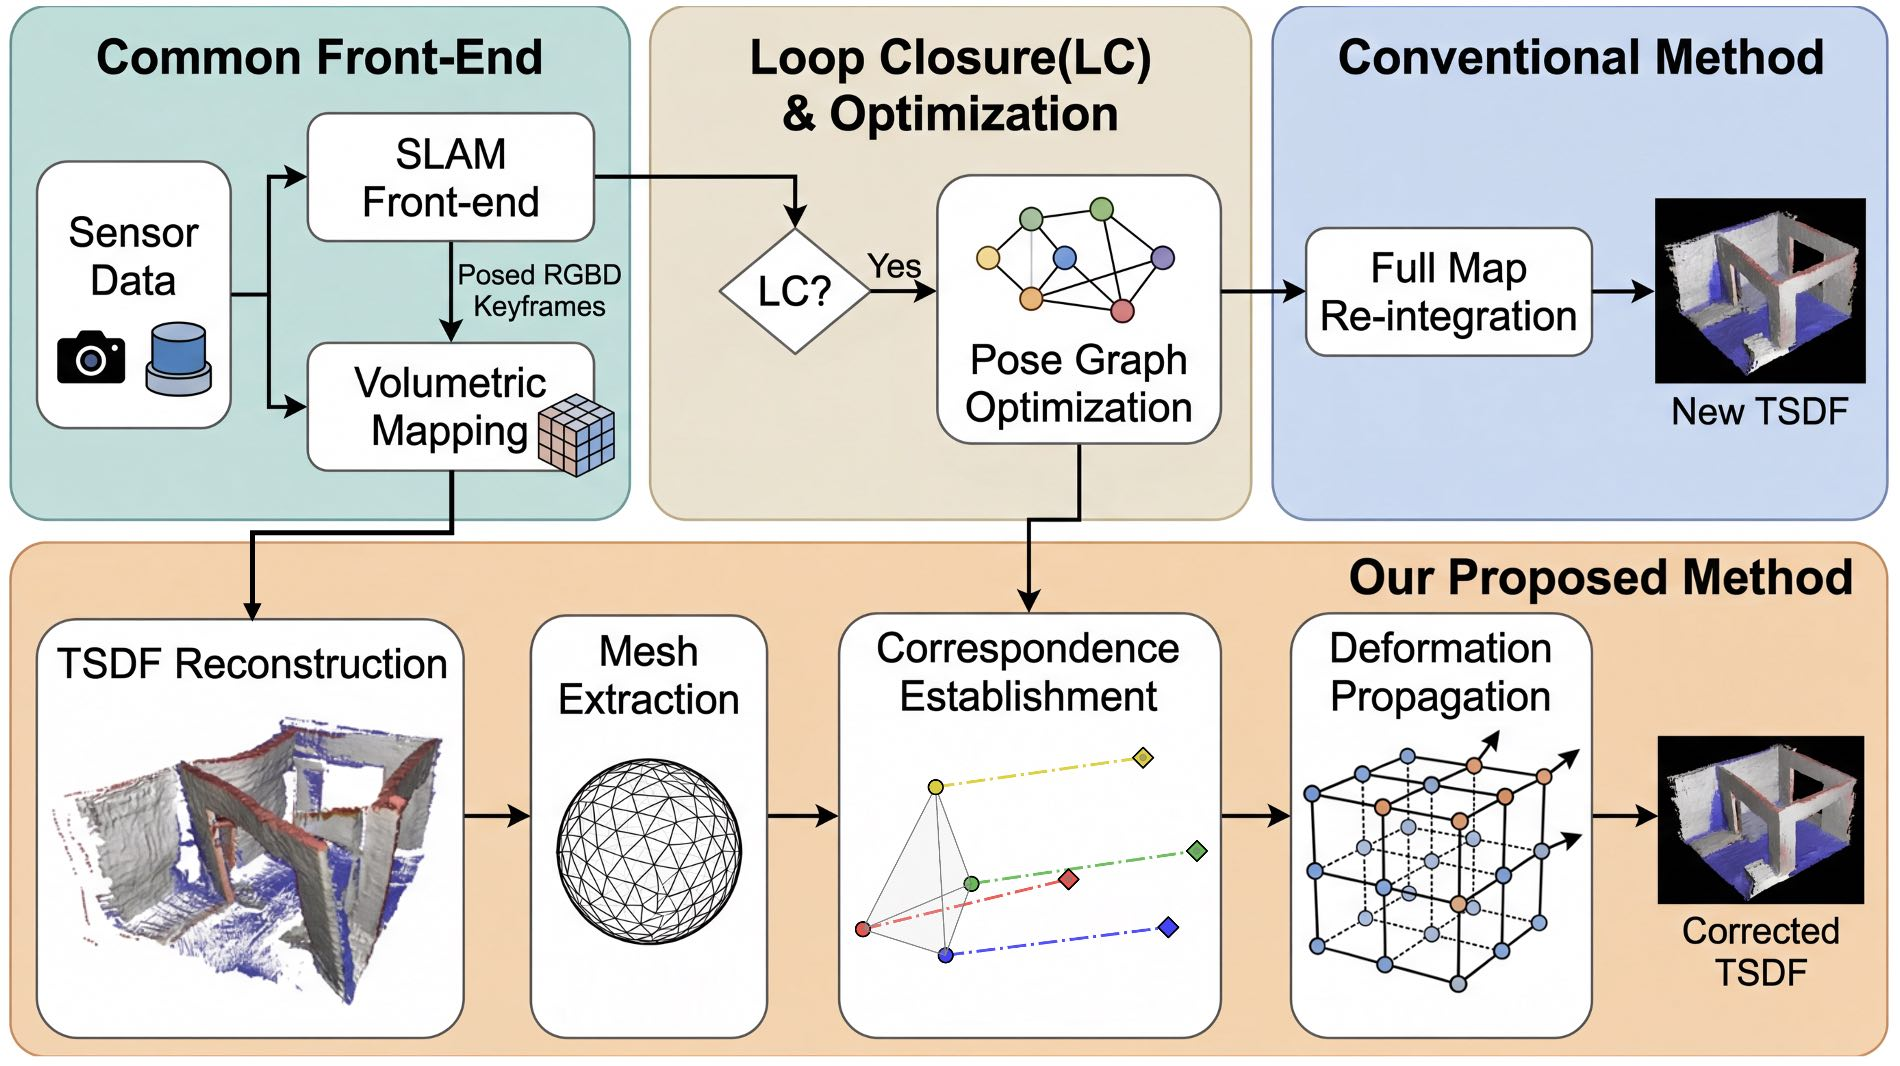
\includegraphics[width=\linewidth]{Figures/pipeline_v5.jpg}
  \caption{WarpVox retains bounded observation support during fusion, resolves
  surface observations after extraction, computes corrected targets from the
  revised trajectory, performs one event-level proxy deformation, and transfers
  source-volume support to the corrected TSDF.}
  \label{fig:pipeline}
\end{figure}

\subsection{Observation Association and Surface Targets}

For RGB-D, pixel $\bar u=[u,v,1]^\top$ with measured z-depth $z_{ij}$ defines
the invariant sensor-frame sample
\begin{equation}
m_{ij}=z_{ij}K^{-1}\bar u,
\qquad
\widetilde m_{ij}=[m_{ij}^\top,1]^\top.
\label{eq:sensor_sample}
\end{equation}
The pre-correction pose projects source vertex $v_j^-$ into frame $i$.
Candidate observations must agree in depth, three-dimensional position, and
viewing direction. Let $n_j^-$ be the source normal, $r_{ij}^-$ the unit
viewing direction in the pre-correction world frame, and $z_{ij}^{\rm proj}$
the projected vertex depth. Define
\begin{equation}
\begin{aligned}
e^g_{ij}
&=\left\|[T_i^-\widetilde m_{ij}]_{1:3}-v_j^-\right\|,\\
e^z_{ij}
&=z_{ij}^{\rm proj}-z_{ij},\\
g_{ij}
&=\left|(n_j^-)^\top r_{ij}^-\right|.
\end{aligned}
\label{eq:association_residuals}
\end{equation}
The effective association reliability is
\begin{equation}
\alpha_{ij}=
\exp\!\left(-\frac{e^g_{ij}}{\sigma_g}\right)
\exp\!\left(-\frac{|e^z_{ij}|}{\sigma_z}\right)
\frac{g_{ij}}{1+z_{ij}^{\rm proj}/z_0},
\label{eq:association_weight}
\end{equation}
subject to a depth-dependent geometric gate and a minimum reliability. LiDAR
uses the analogous construction with spherical projection and radial range.
This is geometric support rather than exact voxel-integration provenance. The
$z_0$ term ranks distant samples during capped association; a separate range
factor below models target reliability after an association has been retained.

After loop closure, each timestamp selects the corresponding corrected pose.
For a missing interior pose, translation is interpolated linearly and rotation
by SLERP over a bounded gap~\cite{shoemake1985slerp}. The invariant sample then
defines the corrected candidate
\begin{equation}
q_{ij}^+=\left[T_i^+\widetilde m_{ij}\right]_{1:3}.
\label{eq:corrected_target}
\end{equation}
This candidate is exact when the static-scene association, calibration, and
corrected pose are valid. Let $\mathcal J_j$ index $\mathcal O_j$, and let
$\rho_{ij}$ be modality-native range, with $\rho_{ij}=z_{ij}$ for RGB-D and
$\rho_{ij}=\|m_{ij}\|$ for LiDAR. We first compute
\begin{equation}
\omega_{ij}=\frac{\alpha_{ij}}{1+\rho_{ij}/\rho_t},
\qquad
\bar q_j=
\frac{\sum_{i\in\mathcal J_j}\omega_{ij}q_{ij}^+}
     {\sum_{i\in\mathcal J_j}\omega_{ij}}.
\label{eq:target_initial}
\end{equation}
The reliability-weighted center is paired with an unweighted median residual
scale so that one high-weight candidate cannot determine both the estimate and
its rejection threshold:
\begin{equation}
\begin{aligned}
\theta_j&=\max\!\left(
\epsilon_t,
\kappa_t\operatorname*{median}_{k\in\mathcal J_j}
\|q_{kj}^+-\bar q_j\|\right),\\
I_j&=\left\{i\in\mathcal J_j:
\|q_{ij}^+-\bar q_j\|\le\theta_j\right\}.
\end{aligned}
\label{eq:target_inliers}
\end{equation}
When fewer than three candidates are available, $I_j=\mathcal J_j$. The final
target and its observable dispersion are
\begin{equation}
v_j^*=
\frac{\sum_{i\in I_j}\omega_{ij}q_{ij}^+}
     {\sum_{i\in I_j}\omega_{ij}},
\qquad
\sigma_j^2=
\frac{\sum_{i\in I_j}\omega_{ij}\|q_{ij}^+-v_j^*\|^2}
     {\sum_{i\in I_j}\omega_{ij}}.
\label{eq:target}
\end{equation}
Only targets passing fixed support and dispersion tests become controls. The
dispersion measures agreement among retained candidates but cannot detect a
mutually consistent yet incorrect association.

\subsection{Event-Level Surface Deformation}

The deformation stage propagates observation-derived motion; it does not infer
correction from shape alone. Let $d_j=v_j^*-v_j^-$ denote an accepted control
displacement. A component-aware local predictor and a median--MAD test reject
isolated displacements before coarsening.

Component-separated spatial clustering~\cite{rossignac1993vertexclustering}
constructs a triangular proxy $\mathcal P^-=(P^-,F_P)$ and selects one QEM
representative~\cite{garland1997qem} per occupied cell. Let
$\pi:V^-\rightarrow P^-$ map source vertices to representatives and
$\mathcal K_a=\{j:\pi(j)=a\}$ collect accepted controls assigned to proxy
vertex $a$. For $\mathcal K_a\neq\emptyset$, the initial proxy displacement and
target are
\begin{equation}
\bar d_a=\frac{1}{|\mathcal K_a|}\sum_{j\in\mathcal K_a}d_j,
\qquad
p_a^{(0)}=p_a^-+\bar d_a.
\label{eq:proxy_initial_target}
\end{equation}
A local-rigid consensus then validates measured proxy targets and supplies
motion where direct support is absent. Weighted orthogonal-Procrustes
fits~\cite{schoenemann1966procrustes} with Welsch
reweighting~\cite{yao2020welsch} predict the local motion; a measured target is
replaced only when it is a gross outlier and a strict same-component majority
supports the replacement. Components without accepted controls inherit a
robust nearby motion through three spatially separated synthetic anchors. Let
$\{p_a^*:a\in\mathcal C_P\}$ denote the resulting accepted or synthesized
proxy targets.

WarpVox performs one event-level proxy ARAP
optimization~\cite{ARAP_modeling:2007,
10.1007/978-3-662-05105-4_2,libigl}:
\begin{equation}
\begin{aligned}
\min_{P^+,\{R_a\in SO(3)\}}\quad
&\frac{1}{2}\sum_{a=1}^{|P^-|}
\sum_{b\in\mathcal N_P(a)}c_{ab}\\[-1mm]
&\left\|(p_a^+-p_b^+)-R_a(p_a^--p_b^-)\right\|^2,\\
\text{s.t.}\quad
&p_a^+=p_a^*,\qquad a\in\mathcal C_P .
\end{aligned}
\label{eq:arap}
\end{equation}
Here $\mathcal N_P(a)$ is the one-ring neighborhood induced by $F_P$, and
$c_{ab}=c_{ba}$ are symmetric cotangent-derived weights; the factor $1/2$
removes double counting. Reliability screening and local consensus decide which
controls survive and where they lie. Once accepted, controls are imposed
exactly so that ARAP does not attenuate the supplied trajectory correction. The
standard local--global iterations solve this single event-level optimization.

Proxy displacement is transferred to $V^-$ by topology-local interpolation. A
local bounded-distortion pass~\cite{sorkine2004laplacian,aigerman2013bounded}
harmonically repairs isolated failures and omits only faces that remain invalid
under fixed dimensionless tests. The retained source and warped surfaces
therefore satisfy
\begin{equation}
\bar{\mathcal M}^-=(\bar V^-,\bar F),
\qquad
\mathcal M^+=(\bar V^+,\bar F),
\qquad
\bar F\subseteq F.
\label{eq:retained_topology}
\end{equation}
Deformation accuracy is therefore governed by target correctness and surface
coverage; neither is independently certifiable without stronger scene
assumptions.

\subsection{Source-Supported TSDF Reconstruction}

The warped surface supplies the corrected zero set~\cite{sussman1999redistancing},
while the source TSDF supplies observed-space semantics. For output voxel center
$x$, a closest-triangle query~\cite{10.1145/2601097.2601199} on $\mathcal M^+$
returns face $f$, closest point $q^+$, and barycentric coordinates $\beta$.
Shared face indices locate the corresponding source point
\begin{equation}
q^-=\sum_{k\in f}\beta_k\bar v_k^-.
\label{eq:source_correspondence}
\end{equation}
Let
\begin{equation}
R_f^\pm=
\begin{bmatrix}
t_{f,1}^\pm & t_{f,2}^\pm & n_f^\pm
\end{bmatrix}\in SO(3)
\label{eq:triangle_frames}
\end{equation}
be consistently oriented orthonormal frames of the corresponding source and
warped triangles. The first tangent follows the same indexed edge and
$t_{f,2}^\pm=n_f^\pm\times t_{f,1}^\pm$. A piecewise local-rigid pullback,
motivated by deformation transfer~\cite{sumner2004deformationtransfer}, maps
$x$ to the source volume:
\begin{equation}
\Psi_f(x)=q^-+R_f^-(R_f^+)^\top(x-q^+),
\qquad x^-=\Psi_f(x).
\label{eq:inverse_map}
\end{equation}
This preserves tangential and normal offsets relative to the corresponding
triangles. With trilinear source samples $\widetilde\Phi^-$ and
$\widetilde w^-$, define
\begin{equation}
\begin{aligned}
r^+(x)&=\|x-q^+\|,\qquad d^+(x)=\min\!\left(\tau,r^+(x)\right),\\
\Omega_{\rm tr}&=\left\{x:\widetilde w^-(\Psi_f(x))>0\right\}.
\end{aligned}
\label{eq:transferred_support}
\end{equation}

Let $\Omega_{\rm fb}\subseteq\mathbb R^3\setminus\Omega_{\rm tr}$ contain
bounded unsupported interpolation holes connected to $\Omega_{\rm tr}$ but not
incident to an open mesh boundary. Its finite fallback weight is
\begin{equation}
w_{\rm fb}(x)=
\begin{cases}
1, & r^+(x)\le0.5s,\\
(1.5s-r^+(x))/s, & 0.5s<r^+(x)\le1.5s,\\
0, & r^+(x)>1.5s.
\end{cases}
\label{eq:fallback_weight}
\end{equation}
The warped normal is oriented to preserve the source TSDF sign convention, so
\begin{equation}
s_f^+(x)=\operatorname{sgn}\!\left((x-q^+)^\top n_f^+\right).
\label{eq:fallback_sign}
\end{equation}
Define $\Omega^+=\Omega_{\rm tr}\cup\Omega_{\rm fb}$ and
$\Phi^+:\Omega^+\rightarrow[-\tau,\tau]$ by
\begin{equation}
\Phi^+(x)=
\begin{cases}
\operatorname{sgn}\!\left(\widetilde\Phi^-(\Psi_f(x))\right)d^+(x),
& x\in\Omega_{\rm tr},\\
s_f^+(x)d^+(x),
& x\in\Omega_{\rm fb}.
\end{cases}
\label{eq:hybrid_tsdf}
\end{equation}
The output weight is
\begin{equation}
w^+(x)=
\begin{cases}
\widetilde w^-(\Psi_f(x)), & x\in\Omega_{\rm tr},\\
w_{\rm fb}(x), & x\in\Omega_{\rm fb},\\
0, & \text{otherwise}.
\end{cases}
\label{eq:hybrid_weight}
\end{equation}
Any fallback extension that introduces a new sign crossing is rejected. Outside
$\Omega^+$, zero weight makes the stored distance immaterial. The resulting
$(\Phi^+,w^+)$ is serialized in the native Voxblox TSDF format; its MC mesh is
used only for visualization and evaluation.

\subsection{Complexity and Scope}

Let $A=|\mathcal A|$, $P=|P^-|$, and $X^+$ be the numbers of active support
cells, proxy vertices, and allocated output voxels. At fixed resolution, MC
produces a constant number of surface elements per active cell, so
$|V^-|=O(A)$. The streaming and resolved correction states satisfy
\begin{equation}
S_{\rm stream}=O(n_cA),
\qquad
S_{\rm corr}=O(n_vA).
\label{eq:state_complexity}
\end{equation}
Because each source vertex queries a fixed stencil, association resolution and
target aggregation require $O((n_c+n_v)A)$. The complete correction cost is
\begin{equation}
\begin{aligned}
C_{\rm corr}={}&O((n_c+n_v)A)+C_{\rm ARAP}(P,F_P)\\
&+C_{\rm vol}(X^+,\bar F),
\end{aligned}
\label{eq:complexity}
\end{equation}
where $C_{\rm vol}$ is the accelerated closest-triangle reconstruction cost. In
the streaming realization, accumulated frame count $N$ does not appear:
bounded support replaces history-dependent replay, while the remaining work
follows the active surface, proxy, and output volume.
